% !TEX root =  lectures.tex
\documentclass[12pt]{article}
\usepackage{graphicx}
\usepackage[
        pdfencoding=auto,%
        pdftitle={Notes on Statistical Mechanics},%
        pdfauthor={Scott Pratt},%
        pdfstartview=FitV,%
        colorlinks=true,%
        linkcolor=blue,%
        citecolor=black, %
        urlcolor=blue]{hyperref}
%\usepackage{pdfsync}
\usepackage{amssymb}
\usepackage{amsmath}
\usepackage{bm}
\numberwithin{equation}{section} 
\numberwithin{figure}{section} 
\usepackage[small,bf]{caption}

%\usepackage{fontspec}
\usepackage{textcomp}
\usepackage{graphicx}
\usepackage{color}
\usepackage{fancyhdr}
\usepackage{bm}
\newcommand\eqnumber{\addtocounter{equation}{1}\tag{\theequation}}

\newcounter{examplecounter}
\setcounter{examplecounter}{0}
\newcommand{\example}[1]{\begin{samepage}
\stepcounter{examplecounter}{\noindent\rule{\textwidth}{1pt}\nopagebreak\\ \bf Example \arabic{section}.\arabic{examplecounter}:}~--~{\bf #1}\\
\end{samepage}
}

\newcommand{\exampleend}{
\begin{samepage}
\nopagebreak\noindent\rule{\textwidth}{1pt}
\end{samepage}}

\newcommand{\aside}[1]{\begin{samepage}
\hrule
{\bf Aside:~}{\bf #1}\\
\end{samepage}
}
\newcommand{\asideend}{
\begin{samepage}
\nopagebreak\noindent\rule{\textwidth}{1pt}
\end{samepage}}

\newcommand{\unity}{\mathbb{I}}

\usepackage[T1]{fontenc}
%\renewcommand*{\sfdefault}{Berenis}
%\renewcommand*{\rmdefault}{Berenis}
\renewcommand*{\sfdefault}{ppl}
\renewcommand*{\rmdefault}{ppl}
%\renewcommand*{\sfdefault}{Bookman}
%\renewcommand*{\rmdefault}{Bookman}

%\pagestyle{empty}
\textwidth 7.0in
\hoffset -0.8in
\textheight 9.2in
\voffset -1in

\pagestyle{fancy}             % page layout
\newcommand{\TheShortTitle}{}
\newcommand{\ShortTitle}[1]{\renewcommand{\TheShortTitle}{#1}}
\fancyhead[LO,RE]{\slshape \TheShortTitle}
\fancyhead[LE,RO]{\slshape \leftmark}

\usepackage{colortbl}
\newcommand{\cc}[1]{\cellcolor{#1}}
\definecolor{lightred}{rgb}{1,0.5,0.6}
\definecolor{lightblue}{rgb}{0.6,0.8,1.0}

\hyphenation{Schr\"odin-ger}

\usepackage{comment}
\parskip 4pt
\parindent 0pt

%\newcommand{\bm}{\boldmath}
\boldmath

% for the banner across the tops of pages 2-
\ShortTitle{BEST SAMPLER}

\begin{document}

\section{Testing Bulk Viscous Corrections}

Bulk viscous corrections to the stress-energy tensor,
\begin{align*}\eqnumber
\Pi=\frac{T_{xx}+T_{yy}+T_{zz}}{3}-P(\rho,\epsilon),
\end{align*}
are non-zero whenever the spatial components of the stress-energy tensor, $T_{ij}$, do not exactly match the expectation for an equilibrated system at a specified energy and charge density, $P\delta_{ij}$. A variety of non-equilibrium effects contribute to $\Pi$. Examples are:
\begin{itemize}
\item The mean field being out of equilibrium
\item Correlations in coordinate space not reaching equilibrium (only matters if there are interactions between particles)
\item Chemical non-equilibrium
\item Kinetic non-equilibrium
\end{itemize}
Given that we are matching to a non-interacting gas, the first two items are irrelevant. The last contribution, chemical non-equilibrium, disappears if one replaces $P(\epsilon,\rho)$ with $P(\epsilon,\vec{n})$, where $n_i$ is the density of species $i$. For our applications, chemical rates are MUCH slower than kinetic equilibration rates or the expansion rates, thus it makes sense for the chemical compositions modeled dynamically, and not modeled as a bulk viscous effect. This leaves only kinetic equilibrium as the source of bulk viscosity for the BEST sampler. 

The bulk viscous correction, $\Pi$, is caused by the expansion rate, $\nabla\cdot\vec{r}$, not being negligibly small compared to the kinetic equilibration rate $1/\delta\tau$. The relaxation time scale $\delta\tau$ is typically $\approx 2$ collision times. For bulk effects one need only consider how the system behaves under an isotropic expansion. For non-isotropic effects, one considers the shear corrections of the next chapter. 

For an isotropic expansion the energy and number densities fall with time as
\begin{align*}\eqnumber
\partial_t n_i&=-(\nabla\cdot\vec{v})n_i,\\
\partial_t \epsilon&=-(\nabla\cdot\vec{v})(\epsilon+P).
\end{align*}
Here, we model the viscous effects by considering the relaxation time approximation. For some time $t$, we assume that the system was kinetically equilibrated at some time $t-\delta t$. At this earlier time, the system was kinetically equilibrated at a higher temperature than the temperature at $T$ because the system would be cooling. For times between $t-\delta t$ and $t$, the system is assumed to free-stream. For a system with an isotropic expansion rate $\nabla\cdot\vec{v}$ a particle with momentum $\vec{p}_0$, as measured in its local rest frame at time $t-\delta t$ will move to a new fluid element with a velocity closer to its own while it is free streaming. For a time $\delta t$, the momentum in the new local rest frame is
\begin{align*}\eqnumber
\vec{p}&=\vec{p}_0-E_p\delta\vec{v},
\end{align*}
where $\delta\vec{v}$ is the velocity of the new fluid element relative to the velocity of the previous element,
\begin{align*}
\delta\vec{v}&=\frac{1}{3}\nabla\cdot\vec{v}\delta\vec{x}=\frac{1}{3E_p}\nabla\cdot\vec{v}\delta\vec{p}\delta t.
\end{align*}
This gives the following evolution for a free-streaming particle,
\begin{align*}\eqnumber
\label{eq:delp}
\delta\vec{p}&=-\frac{1}{3}(\nabla\cdot\vec{v})\delta t\vec{p},\\
\vec{p}(t)&=\frac{t-\delta t}{t}\vec{p}(t-\delta t),
\end{align*}
where the time dependence denotes that the momentum is being measured in a local frame that depends on time. For a Hubble expansion in flat space, which is the three-dimensional extension of a Bjorken expansion, the expansion rate is $\nabla\cdot\vec{v}=3/\tau$, where $\tau$ is the age of the universe as measured by an observer moving with the fluid. This can be shown to give
\begin{align*}\eqnumber
\vec{p}(\tau)&=\frac{\tau_0}{\tau}\vec{p}(\tau_0).
\end{align*}

For kinetic bulk viscosity, one would then consider how much the stress-energy differs between free-streaming and kinetically equilibrated dynamics. In a Hubble expansion the momenta all scale as $1/\tau$, regardless of whether their motion is relativistic or non-relativistic. For massless particles, the energies all scale as $1/\tau$ as well, and given that the thermalized phase space densities behave as $e^{-E/T}$, a free-streaming expansion, which according to Liouville's theorem maintains constant phase space density, maintains a thermal distribution by simply saying $T(\tau)=T(\tau_0)\tau_0/\tau$. Of course, if the system maintains a thermal distribution, collisions have no effect. Thus, there is no kinetic bulk viscosity for a system of massless particles. For a system of non-relativistic particles, the thermalized phase space density behaves as $e^{-p^2/2mT}$, and it also maintains a thermal phase space density by scaling $T(\tau)=T(\tau_0)(\tau_0/\tau)^2$. Again, for a system of non-relativistic particles, even one with species of varying masses, there is no bulk viscosity. Another way to understand the lack of bulk viscosity is to see that the bulk projection of the stress energy tensor and the energy density are:
\begin{align*}\eqnumber
\Pi&=\int\frac{d^3p}{(2\pi\hbar)^3}f(\vec{p})\frac{p^2}{3E_p},\\
\epsilon&=\int\frac{d^3p}{(2\pi\hbar)^3}f(\vec{p})E_p.
\end{align*}
For non-relativistic particles, $\Pi=\epsilon/3$ for massless particles regardless of how the form for $f(\vec{p})$. For non-relativistic particles, if the density of particles is fixed $\Pi=2(\epsilon-\sum_i m_in)/3$ where the mass and densities of the various species, $m_i$ and $n_i$, are fixed. Again, this does not depend on the form for $f$, as long as the phases space densities for each species integrate to the fixed number density.

For particles whose mass makes them semi-relativistic, there are no scaling relations, and the system can accommodate a bulk viscous contribution. This can be seen by placing all the energy into one particle, which gives $\Pi=(\epsilon-\sum_in_i)/3$ because in a large system the only contribution to the mass-subtracted energy and pressure would the one particle, which would be highly relativistic. The form of the phase space density would certainly be peculiar, peaked at $p=0$, then with a contribution at very large $p$. It is difficult to conjur a physical mechanism that could result in more than a small value of $\Pi$. Significantly more leverage comes from considering a system with a mixture of ultra-relativistic and non-relativistic particles. In such a system one can generate $\Pi$ by moving energy from the heavy species to the light species. This is precisely what happens during free streaming. In that case the non-relativistic particles cool much faster, as their characteristic temperatures fall as $\tau^2$ while the temperatures fall as $1/\tau$ for massless particles. Indeed, hadron gases feature a mixture of particles with masses much greater than the temperature and pions, whose thermal velocities are in the neighborhood of 90\% of the speed of light. However, as will be shown later in this study, it is unlikely one would generate bulk viscous pressures where $\Pi$ is more than a percent or so of the equilibrated pressure. 

For the BEST sampler, the goal is generate particles consistent with the density for each species $n_i$, the overall energy density and the given stress-energy tensor, all of which are given by the output of the hydrodynamics module, which defines the hyper-surface. To this end, we consider what $\Pi$ would result from a system with a given value of $\nabla\cdot\vec{v}\delta t$. We assume that the chemistry is at the equilibrated value at time $t$ according to a temperature $T$ and chemical potentials $\vec{\mu}$, but that the kinetic distribution was generated by creating a thermal distribution at a temperature $T+\delta T$, then scaling each momentum by the factor
\begin{align*}\eqnumber
\vec{p}(t)&=R_p\vec{p}(t-\delta t),\\
R_p&=\frac{1}{1+(\nabla\cdot\vec{v}\delta t)/3}.
\end{align*}
The change in temperature $\delta T$ and the factor $(\nabla\cdot\vec{v}\delta t)$ are treated as an unknown small parameters, which are adjusted to match two conditions. First one wishes to reproduce a small bulk viscosity $\delta\Pi$, and secondly the energy density, $\epsilon$, must be the same after first raising the temperature, then scaling down the momentum. This is accomplished by first solving for the factors $A$ and $B$, defined by 
\begin{align*}\eqnumber
\Pi&=A(\nabla\cdot\vec{v})\delta t,\\
\delta T&=B(\nabla\cdot\vec{v})\delta t,
\end{align*}
using thermal arguments. Once this is done the altered temperature and momentum scaling factors are
\begin{align*}\eqnumber
\delta T&=\frac{B}{A}\Pi_{\rm hydro},\\
R_p&=\frac{1}{1+\Pi_{\rm hydro}/(3A)},
\end{align*}
where $\Pi_{\rm hydro}$ is the bulk viscous pressure from the hydrodynamics model. The coefficients $A$ and $B$ are found by thermodynamic relations. The energy density constraint comes from requiring that the increased energy from heating up an element by $\delta T$ is balanced by the work done in expanding according to $\nabla\cdot\vec{v}\delta t$. From keeping the energy fixed,
\begin{align*}\eqnumber\label{eq:Acoeff}
0&=\left.\frac{\partial\epsilon}{\partial T}\right|_{n_i}\delta T-P\nabla\cdot\vec{v}\delta t\\
&=\sum_h n_h\partial_T\left(\frac{\int d^3p~Ee^{-E_p/T}}{\int d^3p~e^{-E_p/T}}\right)-P\nabla\cdot\vec{v}\delta t,\\
&=\sum_h\left(\partial_T|_\mu\epsilon_h-\frac{1}{T^2}\frac{\epsilon_h^2}{n_h}\right)\delta T
-P\nabla\cdot\vec{v}\delta t,\\
A&=\frac{P}{\partial_T|_\mu\epsilon-\frac{1}{T^2}\sum_h\epsilon_h^2/n_h}.
\end{align*}
Next, the non-equilibrated bulk pressure due to the free-streaming expansion is 
\begin{align*}\eqnumber
\delta\Pi&=\sum_h n_h\partial_T\left(\frac{\int d^3p~(p^2/3E_p)e^{-E_p/T}}{\int d^3p~e^{-E_p/T}}\right)\delta T\\
&-\sum_h\int\frac{d^3p}{(2\pi\hbar)^3}e^{-(E_p-\mu)/T}p_i\frac{d}{dp_i}\frac{p^2}{3E_p}(\nabla\cdot\vec{v})\delta t.
\end{align*}
This last expression uses Eq. (\ref{eq:delp}) for the change in the momentum during the free streaming. Using Eq. (\ref{eq:Acoeff}) to eliminate $\delta T$,
\begin{align*}\eqnumber\label{eq:Blambdadef}
B&=-A\epsilon T+\left.\frac{A}{3}\partial_T\epsilon\right|_\mu-\frac{A}{3}\sum_h m_h^2n_h-\frac{2}{3}P+\frac{1}{9}\lambda,\\
\lambda&=\sum_h\int\frac{d^3p}{(2\pi\hbar)^3} e^{-(E_p-\mu)/T}\frac{p^4}{E_p^3}.
\end{align*}
Here, $m_h$ is the mass of the hadron species $h$. The sampling algorithm consists of first generating the species according to the chemistry at the given time, then generating the momenta using the higher temperature, $T+B\Pi/A$. The momenta then scaled down by the factor $1/(1+\Pi/3A)$. 

The method should exactly reproduce the desired deviation of the bulk pressure and not change the energy density to first order in $\Pi$. To see that this is the case, several billion particles were created Monte Carlo according to this prescription. The stress-energy tensor was calculated as 
\begin{align*}\eqnumber
T_{00}&=\frac{1}{V}\sum E_p,\\
T_{ij}&=\frac{1}{V}\sum \frac{p_ip_j}{E_p}.
\end{align*}
Figure \ref{fig:bulktest_mu0} compares the ratio $\sum T_{ii}/3-P$ to the target value of $\Pi$ for several values of $\Pi$. The temperature $T$ was set to 150 MeV, and the chemical potentials were set to zero. It also displays the ratio of the resulting energy density $T_{00}$ to the thermal value $\epsilon$. If the procedure is successful, both ratios will remain at unity. The original energy density never varies more than a tenth of a percent, and the bulk viscous contribution is reproduced to within a few percent. Also illustrated are the generating temperature and the momentum scaling factor. Even though the range of $\Pi/P$ in Fig. \ref{fig:bulktest} never exceeds a percent or so, at which point the generating temperature reaches approximately 50 MeV above the 150 MeV temperature and the momentum scaling factors falls to nearly 0.75. This emphasizes the point that bulk contributions should be small.
\begin{figure}
\centerline{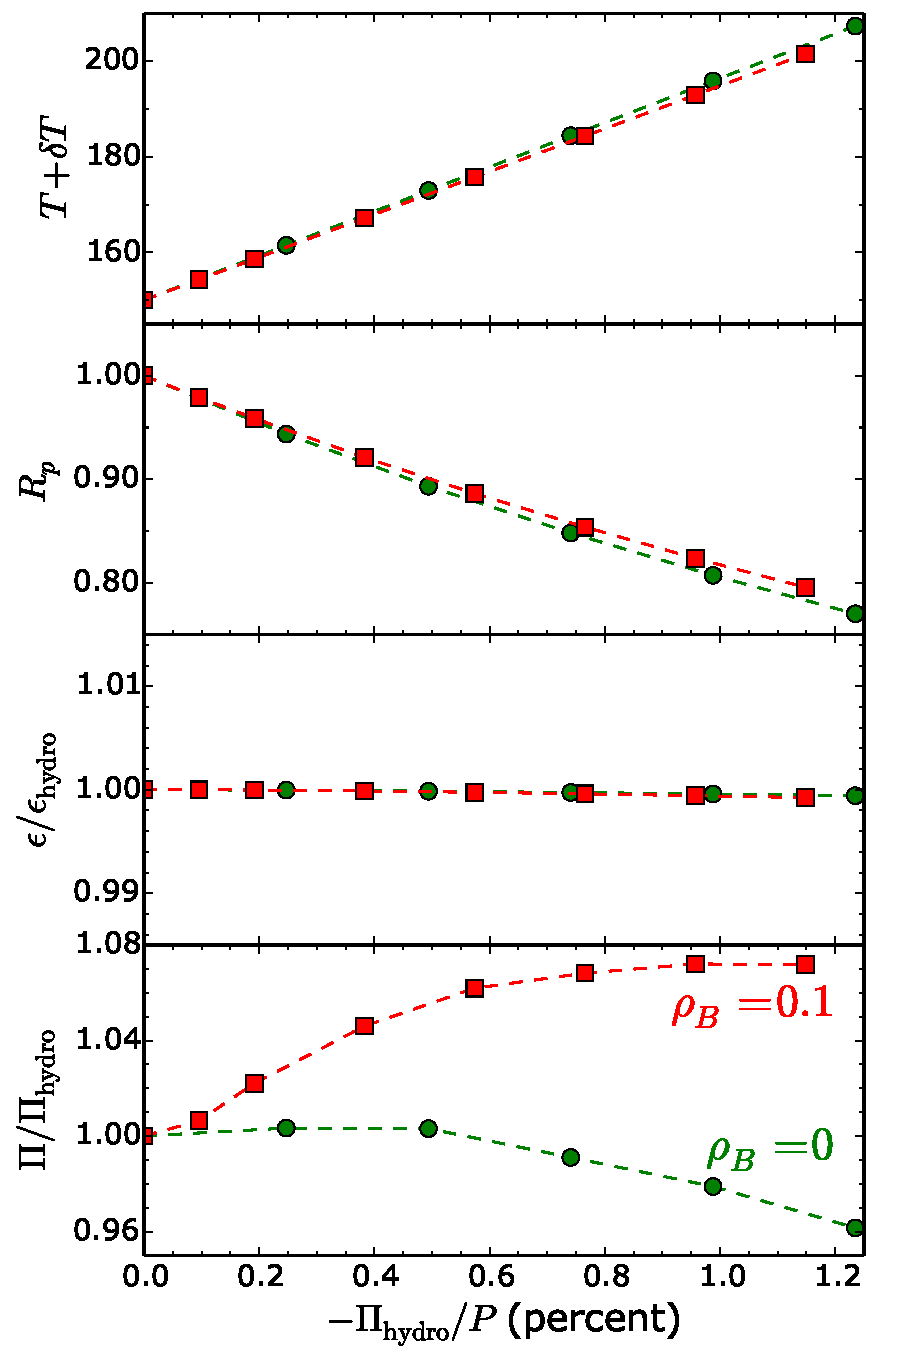
\includegraphics[width=0.6\textwidth]{figs/bulk}}
\caption{\label{fig:bulktest}
The viscous correction to the stress energy was calculated from particles generated by the Monte Carlo procedure outlined in the text, then compared to the target value as a function of the target value. The target value of $\Pi$ is reproduced to within a few percent. The procedure should also reproduce the desired energy density. That is accomplished to better than a tenth of a percent. The procedure involved generating particles at a higher temperature $T+\delta T$, then scaling the momenta by a factor $R_p$. Despite the fact that $\Pi/P$ is only varied from zero to one percent, the required values of $\delta T$ and $R_p$ were substantial. This emphasizes the fact that the bulk viscous contributions for the hadron gas just below hadronization should be small.
}
\end{figure}
To test the procedure for the case where the baryon densities were non-zero, Fig. \ref{fig:bulktest} also shows the same quantities, but calculated with a non-zero baryon density of 0.2 baryons/fm$^3$. The procedure was similarly successful.

As mentioned earlier, during a collisionless expansion the non-relativistic and highly relativistic particles cool at different rates. To understand the degree to which this might influence spectra, the average kinetic energies of nucleons and pions as calculated from the Monte Carlo procedure are displayed in Fig. \ref{fig:EpiEp} as a function of the targeted value of $\Pi$. As expected, the bulk viscous corrections lead to warmer pions and cooler nucleons. The energies were never altered by more than 10\%, which suggests that corrections to spectra for bulk viscosity are modest but perhaps non-negligible.

\section{Shear Viscous Corrections}

Here we compare two corrections. The first was momentum scaling method proposed in \cite{Pratt:2010jt} and the second is just the usual $\delta f$ correction. In the scaling method one generates particles with a given momentum in the fluid frame $\vec{p}^{\rm no~visc}$, then scales the momenta,
\begin{align*}\eqnumber
p_i&=(\delta_{ij}+\pi_{ij}/R_{\rm shear})p^{\rm no~visc.}_j,\\
R_{\rm shear}&=\frac{2\lambda}{15}-2P,
\end{align*}
where $\lambda$ was defined in Eq. (\ref{eq:Blambdadef}). The second is to use the following correction to the phase space density,
\begin{align*}
\delta f&=f-f_{\rm isotropic}=-\frac{p_i\pi_{ij}p_j}{E_pR_{\rm shear}T}f.
\end{align*}
For large momenta, the scaling method will lead to negative values of the phase space density. In the algorithm used here, particles are generated with thermal weights, then the directions of the momenta are chosen according to the weight $(f+\delta f)/f$. A keep-or-reject algorithm calculates $f=(f_{\rm isotropic}+\delta f)/f_{\rm max}$, where $f_{\rm max}$ is the value of $f+\delta f$ using the direction of $\vec{p}$ that maximizes the phase space density. By comparing $f/f_{\rm isotropic}$ to a random number, and discarding directions where the random number exceeds the ratio, a distribution of directions is generated consistent with the overall phase space density. This fails if there are directions for which the phase space density becomes negative, as can happen for large momentum. In this implementation, if $f/f_{\rm isotropic}$ is negative, the direction is always discarded.

Both methods should reproduce the desired behavior for small $\pi$, and in fact can be shown to be equivalent in that limit. For larger $\pi$ they begin to fail to exactly reproduce $\pi$, and the scaling method will also begin to fail to reproduce the energy density. Figure \ref{fig:shear_scaling} shows the accuracy of the scaling solution, essentially recreating the studies in \cite{Pratt:2010jt}. Here, a hydrodynamic hyper-element was sampled where the stress energy tensor is $\pi_{i\ne j}=0$, $\pi_{xx}=\pi_{yy}=-\pi_{zz}$ and with $\pi_{zz}$ set to some fixed value. The value was chosen to be negative to correspond to the expected conditions in a Bjorken expansion. The value of the $\pi_{zz}$ from the generated particles,
\begin{align*}\eqnumber
\pi_{zz}&=\frac{1}{V}\sum_i\frac{p_{i,z}^2}{E_{i}}-P,
\end{align*}
was divided by the hydrodynamic input valuem $\pi^{\rm(hydro)}_{zz}$. If this ratio is unity, the method is successful. 
\begin{figure}
\centerline{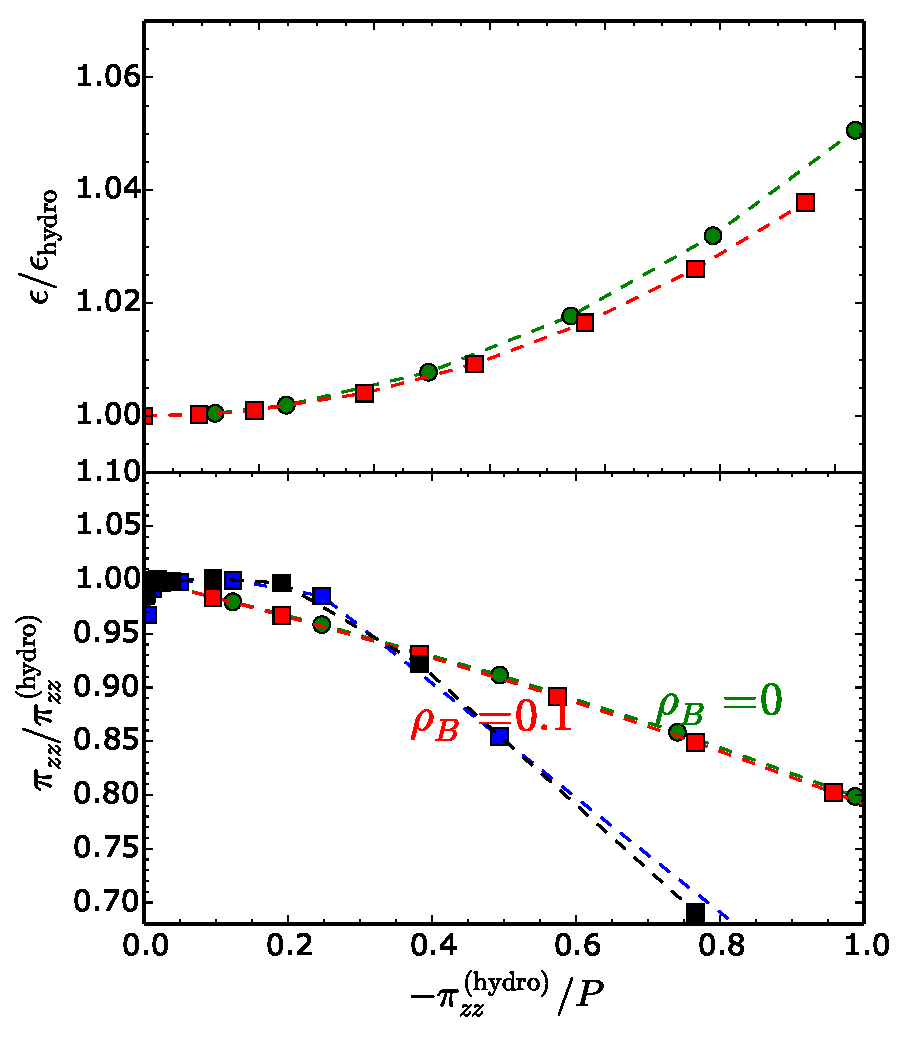
\includegraphics[width=0.6\textwidth]{figs/shear}}
\caption{\label{fig:shear_scaling}
The value of the $zz$ component of the stress-energy tensor is divided by the desired hydrodynamic input as a function of the desired input divided by the pressure. In the linear approximation, the ratio should approach unity as $\pi^{\rm hydro}_{zz}$ vanishes. The energy density should also be unchanged, but for the scaling method does vary from unity for large $\pi/P$. Both the scaling an $\delta f$ methods behave correctly for small shear corrections. For the scaling method, the overall energy conservation fails at the one percent level once $|\pi_{\rm zz}/P|$ exceeds 1/2. At that point the generated $\pi_{zz}$ misses the target by nearly 10\%. The $\delta f$ method exactly reproduces the desired energy density for any $\pi$, but is less successful than the scaling method at reproducing the desired $\pi_{zz}$ for larger anisotropies. Success varied little with different baryon densities. The red/green lines are for the scaling solutions and the blue/black are for the $\delta f$ method.}
\end{figure}
\begin{thebibliography}{99}
%\cite{Pratt:2010jt}
\bibitem{Pratt:2010jt}
S.~Pratt and G.~Torrieri,
%``Coupling Relativistic Viscous Hydrodynamics to Boltzmann Descriptions,''
Phys. Rev. C \textbf{82} (2010), 044901
doi:10.1103/PhysRevC.82.044901
[arXiv:1003.0413 [nucl-th]].
%35 citations counted in INSPIRE as of 29 Apr 2020
\end{thebibliography}
\end{document}
